\documentclass[a4paper,11pt,fleqn]{scrartcl}%fleqn pour aligner les equations à gauche
\usepackage{../../Styles/Cours}


\newcommand{\chnum}{Chapitre 05}
\newcommand{\chtitle}{Mise en \oe uvre d'un titrage colorimétrique}
\newcommand{\dtype}{Cours}

\begin{document}
	\maketitle
    Le Lugol est une colution antiseptique utilisée à différentes concentrations. Celle-ci est composée de diiode \ce{I2 (aq)} qui lui confère sa couleur brun-orange caractéristique.
    \begin{problematique}
        Comment peut-on déterminer la concentration en diiode d'une solution de Lugol ?
    \end{problematique}

    \noindent \begin{minipage}{0.49\linewidth}
        \begin{documentboxenv}{Principe d'un titrage}
        \begin{center}
            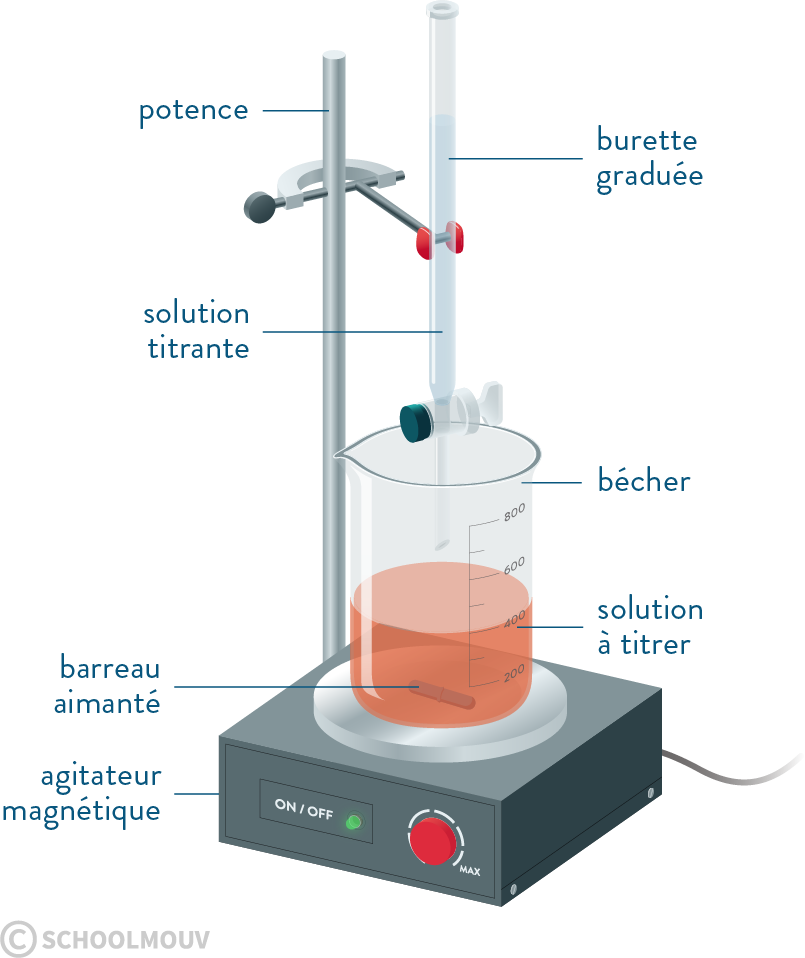
\includegraphics[width=0.85\linewidth]{Ressources/schema_titrage.png}
        \end{center}
        Un titrage est une technique mettant en jeu une transformation chimique rapide et totale entre : \begin{itemize*}
            \item Un réactif titrant de concentration connue
            \item Un réactif titré de concentration à déterminer
        \end{itemize*}
        Dans un titrage avec suivi colorimétrique, un changement de couleur est observé à l'équivalence.
    \end{documentboxenv}
    \end{minipage}
\begin{minipage}{0.49\linewidth}
    \begin{protocole}
        Réaliser un titrage rapide pour estimer le volue versé à l'équivalence $V_E$, puis un second plus précis pour avoir le volume équivalent à la goutte près.
        \begin{enumerate}
            \item Dans un erlenmeyer, introduire $V_1 = \SI{10,0}{mL}$ de la solution antiseptique.
            \item Ajouter à l'aide de la burette graduée la solution de thiosulfate de sodium de concentration effective en ion thiosulfate [\ce{S2O3^2-}] = \SI{1,0E-2}{mol.L^{-1}} tout en agitant jusqu'à obtenir une teinte jaune pâle persistante.
            \item Ajouter une pointe de spatule de thiodène.
            \item Continuer à verser la solution de thiosulfate de sodium jusqu'à l'équivalence du titrage.
        \end{enumerate}
    \end{protocole}
    \begin{documentboxenv}{Informations générales}
    \begin{itemize*}
        \item Couples oxydant/réducteur mis en jeu et couleur des espèces en solution : diiode. (brun) \ce{I2 (aq)}, ion thiosulfate (incolore) \ce{S2O3^2-}, ion iodure (incolore) \ce{I-}.
        \item Le thiodène révèle la présence de diiode en donnant à la solution une coloration bleue. l'un ou l'autre sera ajouté juste avant l'équivalence pour faciliter son repérage.
    \end{itemize*}
    \end{documentboxenv}
\end{minipage}
    
    

    \begin{question}
        \begin{enumerate}
            \item Indiquer les réactifs impliqués dans la réaction chimique support du titrage.
            \item Définir l'équivalence et préciser le changement de couleur attendu.
            \item Mettre en place le montage du titrage, suivre le protocole et noter la valeur du volume versé à l'équivalence.
            \item Dresser le tableau d'avancement de la transformation chimique du titrage puis établir la relation entre les quantités de matière des réactifs qui ont été introduits à l'équivalence.
            \item Calculer la quantité de matière, puis la concentration en quantité de matière $C_1$ en diiode de la solution titrée. À partir des valeurs de concentration du groupe, calculer la concentration moyenne et l'écart-type expérimental.
            \item Proposer une méthode pour déterminer dans un cas général la concentration en quantité de matière d'une espèce en solution.
        \end{enumerate}
    \end{question}
\end{document}